% Short paper, ACM single column review format.
% For the double blind conference submission, change the first line to
%   \documentclass[manuscript,review,anonymous]{acmart}
\documentclass[manuscript,review]{acmart}

\settopmatter{printacmref=false}
\setcopyright{none}
\renewcommand\footnotetextcopyrightpermission[1]{}
\acmConference[AH '27]{Augmented Humans International Conference 2027}{March 7--10, 2027}{Colombo, Sri Lanka}

\usepackage{booktabs}
\usepackage{multirow}

\begin{document}

\title[Communic-aid]{Communic-aid: Learning How Much Evidence to Ask For in Gaze-Based Messaging on a Commodity iPhone}

\author{Vandya Bisaria}
\author{Mansie Singh}
\author{Sinngam Khaidem}
\author{Manan Solanki}
\affiliation{%
  \institution{Indian Institute of Technology Gandhinagar}
  \city{Gandhinagar}
  \country{India}}

\renewcommand{\shortauthors}{Bisaria et al.}

\begin{abstract}
Gaze is often the most reliable input left to people with severe motor impairments, but gaze
interfaces still force a single trade off on every action: a long dwell is slow, a short dwell
selects things by mistake, and a fixed confirmation step is either too weak for a call or too
tedious for a letter. We present Communic-aid, a hands-free messaging interface that uses only an
iPhone with a TrueDepth camera as its sensor. The phone streams gaze, head pose, blinks, eyebrow
raises and a spoken confirmation word to a laptop, which runs a chat app with calls, messages and
a gaze keyboard. Our central idea is that the interface should learn how much evidence to ask for
before it acts, for each person, each context and each level of risk. Every action belongs to one
of four risk tiers with an accident cost. A dwell learner sets the dwell time from implicit
feedback (undos, quick backspaces, abandoned looks and stray glances) using Thompson sampling, and
a contextual bandit chooses which second signal, if any, to ask for on risky actions. A
preliminary study with two able-bodied participants shows that the learner shortened the dwell
from 1500 ms to about 1200 ms within one session, with two accidents in 146 selections, both on
undoable letters and none on risky actions, that the router adapted its choice of confirmation
signal to each participant within a session, and that a grouped
keyboard with large targets was 1.5 to 2.8 times faster than QWERTY for gaze typing. We describe
the planned within-subject comparison against a fixed baseline, including a participant with a
motor impairment.
\end{abstract}

\begin{CCSXML}
<ccs2012>
<concept>
<concept_id>10003120.10011738.10011775</concept_id>
<concept_desc>Human-centered computing~Accessibility technologies</concept_desc>
<concept_significance>500</concept_significance>
</concept>
<concept>
<concept_id>10003120.10003121.10003128</concept_id>
<concept_desc>Human-centered computing~Interaction techniques</concept_desc>
<concept_significance>300</concept_significance>
</concept>
</ccs2012>
\end{CCSXML}
\ccsdesc[500]{Human-centered computing~Accessibility technologies}
\ccsdesc[300]{Human-centered computing~Interaction techniques}

\keywords{gaze interaction, adaptive dwell time, multimodal confirmation, contextual bandit,
motor impairment, augmentative and alternative communication, commodity hardware}

\maketitle

\section{Introduction}

For many people with ALS, muscular dystrophy, cerebral palsy or spinal cord injury, the eyes
remain controllable long after the hands do. Gaze interfaces build on this, but they inherit the
Midas touch problem \cite{jacob1990}: the eyes are always looking at something, so the interface
cannot tell a look that means ``do this'' from a look that means ``I am reading''. The standard
answer is a dwell time. A long dwell is safe and slow; a short dwell is fast and causes accidental
selections. Both kinds of error hurt, but not equally. Accidentally typing a letter costs one
backspace. Accidentally calling someone or deleting a message costs far more.

Existing systems address parts of this. Adaptive dwell methods adjust the dwell to the typist
\cite{majaranta2009, mott2017, narkar2024}, and multimodal methods add a second channel to
confirm a selection \cite{cha2026, namnakani2025}. Our literature review found three gaps that
these systems leave open. First, confirmation is uniform: low cost and high cost actions face the
same bar. Second, adaptive dwell methods mostly learn from explicit signals, and treat a false
selection and a missed selection as equally bad. Third, no system we found chooses the
confirmation modality itself from experience, even though people differ greatly in which signals
they can produce reliably \cite{severitt2026, zhang2026}. Specialised eye trackers also remain
costly and obtrusive, which our interviewees and prior work identify as a barrier
\cite{zhang2017, meena2025}.

We present Communic-aid, which treats these as one problem: \emph{how much evidence should the
interface ask for before it acts?} It answers per person, per context and per level of risk,
and it learns the answer from how the person actually uses it. Our contributions are:
\begin{itemize}
  \item A hands-free messaging system whose only sensor is an iPhone with a TrueDepth camera,
        combining gaze or head pointing with four confirmation signals: blink and hold, raised
        eyebrows, a spoken ``go'', and an optional switch.
  \item Risk tiers that give every action an accident cost, so the strength of confirmation
        scales with what an error would cost.
  \item A dwell learner that sets the dwell time per tier and context from implicit feedback
        alone, with asymmetric steps that lengthen quickly after accidents and shorten slowly.
  \item A contextual bandit that ranks confirmation modalities from past interactions and asks
        for the one most likely to succeed at the lowest effort.
  \item Preliminary results from two able-bodied participants, and a study plan for the
        comparison against a fixed baseline.
\end{itemize}

\section{Related Work}

\textbf{Dwell and the Midas touch.} Dwell selection is the default for gaze input, and the right
dwell depends on the person and the task \cite{paulus2021}. Majaranta et al.\ let typists adjust
the dwell themselves and saw speed rise with practice \cite{majaranta2009}. Mott et al.\ varied
the dwell per key with the probability of the next letter \cite{mott2017}. GazeIntent adapts the
dwell with a learned model of intent and found that most returning users preferred the
personalised version \cite{narkar2024}, and Meena et al.\ adapt a multimodal keyboard over time
\cite{meena2019}. These methods tune one threshold for all actions, and most learn from explicit
corrections. Communic-aid learns from implicit outcomes and weighs accidents by the cost of the
action.

\textbf{Second signals.} Pairing gaze with another channel reduces accidental selections:
silent speech for people with ALS \cite{cha2026}, gestures paired with dwell on mobile devices
\cite{namnakani2025}, and anomaly detection that stops likely errors \cite{severitt2026}. Facial
gestures can be personalised to the user \cite{manzoni2024}, but recognisers show accuracy gaps
for people with motor impairments \cite{zhang2026}. This argues against fixing one confirmation
signal in advance, and for choosing it from what works for each person, in the spirit of
ability-based design \cite{wobbrock2011}.

\textbf{Commodity hardware.} GazeSpeak showed that a smartphone camera can support gaze gesture
communication for people with motor disabilities \cite{zhang2017}, and webcam keyboards bring gaze
typing to low resource settings \cite{meena2025}. Since 2024 iOS also includes system eye
tracking with dwell control \cite{apple2024}. Communic-aid uses the phone differently: as a
sensor that streams gaze, head pose, facial blendshapes and speech to a larger screen, so that
one device provides both pointing and several confirmation signals.

\section{Formative Input}

We interviewed three people with motor impairments (muscular dystrophy, cerebral palsy, and a
locomotor disability), using questions adapted from the WebAIM survey \cite{webaim2013}. Together
with the literature, they shaped five requirements: (1) avoid accidental actions, above all for
calls and deletions; (2) adapt to the individual rather than to an average user; (3) use a second
modality for confirmation, but sparingly, since too many confirmations are tiring; (4) keep the
setup cheap and unobtrusive, with no special hardware; and (5) tolerate involuntary and atypical
movement, including speech that dictation handles poorly. One interviewee already sent voice
notes instead of long texts because typing took too long, which led us to treat typing effort as
a primary cost.

\section{System}

\begin{figure}[t]
  \centering
  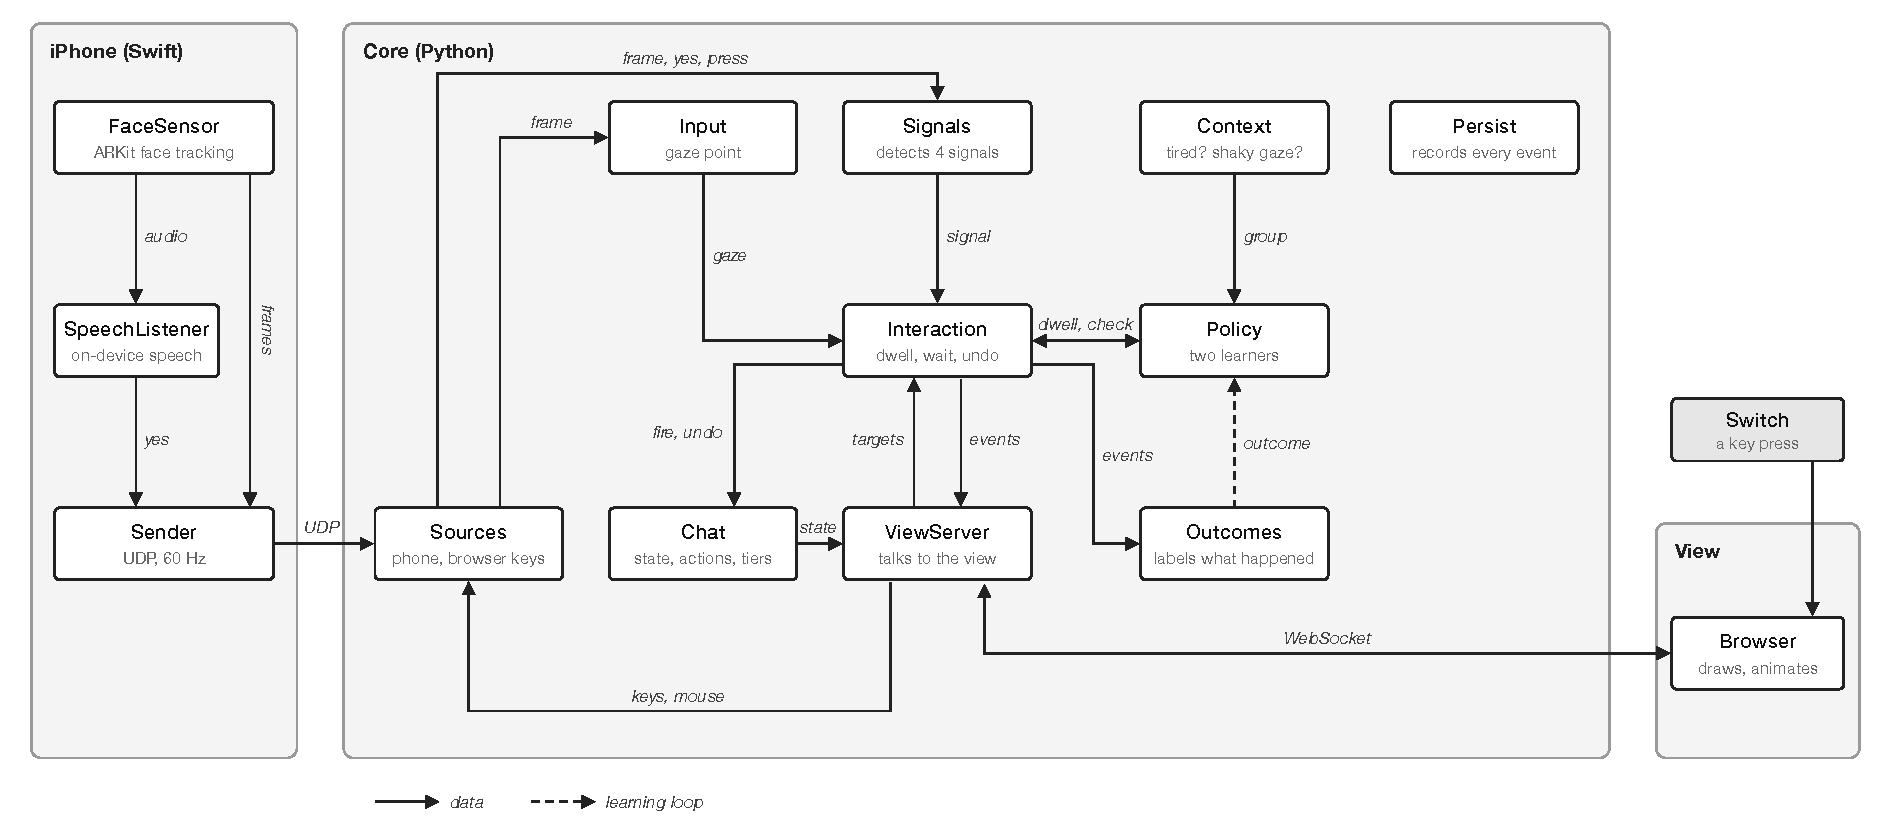
\includegraphics[width=\linewidth]{figures/architecture.pdf}
  \caption{Architecture. The iPhone only senses. The Python core makes every decision: it maps
  gaze to the screen, detects signals, runs the dwell and the confirmation step, labels outcomes
  and updates the two learners. The browser only draws.}
  \Description{Block diagram with three regions. The iPhone sends face frames and a spoken
  confirmation over UDP to a Python core with modules for input, signals, context, interaction,
  policy, outcomes, chat and persistence. The core talks to a browser view over a WebSocket. A
  dashed arrow from outcomes back to policy marks the learning loop.}
  \label{fig:arch}
\end{figure}

\subsection{Sensing with one phone}

The phone sits below the screen, 40 to 60 cm from the face. An iOS app built on ARKit face
tracking sends, at 60 Hz over UDP, the gaze ray and eye position in camera space, the direction
of the nose, and the blink and eyebrow blendshapes. Speech recognition runs on the phone and
listens only for the word ``go''. A Python core on the laptop maps the gaze ray to the screen
with a nine point calibration (a quadratic least squares fit with a small ridge term), smooths it
with an exponential filter, holds it still during blinks, and corrects slow drift using the
centres of buttons the person has just selected. In head pointing mode the same pipeline uses the
nose direction instead of the gaze ray. Signals are detected from the blendshapes: a blink held
for 500 ms, eyebrows raised for 300 ms, or the spoken word. A one time signal check measures each
person's rest and peak levels and sets each threshold halfway between them.

\subsection{Risk tiers}

\begin{table}[t]
  \caption{Risk tiers. The accident cost enters both learners. Tier 0 and 1 actions fire on dwell
  alone; tier 2 and 3 actions add a confirmation step after a short fixed dwell of 1000 ms.}
  \label{tab:tiers}
  \small
  \begin{tabular}{llcl}
    \toprule
    Tier & Actions & Cost & Confirmation \\
    \midrule
    0 & Open a chat, go back, scroll, navigation & 1 & Learned dwell \\
    1 & Letters, word suggestions, Space, Backspace, settings & 2 & Learned dwell \\
    2 & Send, react, end a call & 4 & The router chooses dwell alone or a signal \\
    3 & Call, delete, forward & 8 & Always a signal, chosen by the router \\
    \bottomrule
  \end{tabular}
\end{table}

Every action belongs to one of four tiers (Table~\ref{tab:tiers}). The cost of an accident
doubles with each tier. Undo is always available for 5 seconds through an undo strip on the
screen, so the cost of a tier 0 or 1 accident is a short repair, while a call that has started
cannot be taken back.

\subsection{Labelling outcomes without asking}

The learners never ask the user for feedback. Instead the core labels each look and each
confirmation request from what happens next. A selection that is undone within 5 s, or a letter
that is deleted within 3 s, is an \emph{accident}; otherwise it \emph{worked}. A look that filled
at least half of the dwell, ended, and was followed within 5 s by a fresh selection of the same
button is a \emph{give-up}: the person wanted it but the dwell was too long. Any other unfilled
look is a \emph{stray glance}. For confirmation requests, a signal that arrives is \emph{worked}, a
request abandoned after trying is a \emph{give-up}, and a request that times out with no attempt
at all is \emph{blocked}: the confirmation step stopped an action the person did not want.

\subsection{Context}

Each learner keeps separate statistics for four context groups: rested or tired (more than
20 minutes into the session, or in the evening) crossed with steady or shaky gaze (the recent
spread of gaze on targets more than 1.5 times a steady baseline). Until a group has
enough data of its own, it borrows the pooled data of all groups.

\subsection{Dwell learner}

For tiers 0 and 1, the dwell learner keeps six counts per group: intended and unintended looks,
stray glances and their total duration, and give-ups and the total waiting time. From these it
draws, by Thompson sampling \cite{thompson1933}, a probability $\pi$ that a look is intended (from
a Beta distribution), a mean stray glance length $g$ and a mean patience $p$ (from Gamma
distributions). For each candidate dwell $d$ between 800 and 2000 ms it scores
\[
  V(d) = \pi\left[(1 - G(d))\,(1 - \lambda d) + r_{\text{give-up}}\,G(d)\right] - (1-\pi)\,A(d)\,c_{\text{tier}},
\]
where $A(d) = e^{-d/g}$ is the chance that a stray glance lasts long enough to fire, $G(d) = 1 -
e^{-d/p}$ is the chance that the person gives up first, $\lambda = 0.6$ per second is the cost of
waiting, $r_{\text{give-up}} = -0.5$, and $c_{\text{tier}}$ is the accident cost. The best $d$ is a
target, not a setting: after each selection the dwell moves 5\% of the way towards it, by at most
10 ms when shortening and up to 100 ms when lengthening, so that accidents are corrected quickly
while speed is gained cautiously. The dwell starts at 1500 ms and stays there for the first 20
selections in a group.

\subsection{Modality router}

For tiers 2 and 3, a contextual bandit \cite{li2010} chooses the confirmation step. The arms are
dwell alone (tier 2 only), blink and hold, raised eyebrows, the word ``go'', and a switch. For each
arm, tier and group it keeps a count of the four outcomes (worked, give-up, blocked, accident) and
draws their probabilities from a Dirichlet distribution. The expected value of an arm weighs the
outcomes by their rewards: a worked signal earns $1$ minus its effort, which grows with the
person's average time to produce that signal; a blocked accident earns a small positive reward
proportional to the tier cost; an accident costs the full tier cost. The arm with the highest
sampled value is asked for. The person's preferred signal, chosen in settings, starts with a small
bonus, and a group borrows the pooled counts until it has 20 tries of its own. Because sampling
keeps some uncertainty, a signal that worked poorly early on is still tried occasionally rather
than being ruled out for good.

\subsection{Interface}

The view is a full screen chat app with a chat list, threads, calls, message actions and
settings. A look fills the target button; a confirmation request shows which signal to give and
waits up to 4 seconds. Text entry offers two keyboards: a grouped keyboard with eight large
letter groups (abc, def, \dots, wxyz) where a letter takes two selections, and a QWERTY keyboard
with one selection per letter. Word suggestions appear above both.

\section{Preliminary Study}

\subsection{Method}

Two able-bodied adults (P1, P2) used the system with gaze pointing in the adaptive condition, on
a laptop with the phone mounted below the screen and their heads free to move. After the signal
check and calibration, each used the chat app freely and completed the study tasks: navigating
between chats and settings, composing and sending a message of at least ten letters, making and
ending a call, and deleting a message. P1's session lasted 9 minutes and P2's 24 minutes. Each
then did a typing test: copying a 248 character passage for two minutes, without word
suggestions, three times with each keyboard, grouped first, with a new passage in every run. We
report words per minute ($\text{WPM} = (n-1)/t \times 60/5$ for $n$ characters in $t$ seconds),
accuracy from the edit distance to the passage, and keystrokes per character
\cite{soukoreff2003}. All measures come from the core's event log.

\subsection{Results}

\begin{table}[t]
  \caption{Free use session. Selections exclude undo and redo. Head movement is the distance of
  the eyes from their median position; turning is the angle of the nose from its median direction.}
  \label{tab:session}
  \small
  \begin{tabular}{lrr}
    \toprule
    Measure & P1 & P2 \\
    \midrule
    Session length & 9 min & 24 min \\
    Calibration error & 80 px & 69 px \\
    Selections (tier 0 / 1 / 2 / 3) & 51 (18 / 29 / 2 / 2) & 95 (32 / 51 / 7 / 5) \\
    Accidents & 2 (both tier 1) & 0 \\
    Undos & 2 & 0 \\
    Dwell give-ups & 6 & 11 \\
    Stray glances & 145 & 541 \\
    Confirmation requests on tiers 2 and 3 & 5 & 13 (4 dwell alone) \\
    \quad worked / gave up / accidents & 4 / 1 / 0 & 12 / 1 / 0 \\
    Dwell at end, tier 0 / tier 1 & 1216 / 1333 ms & 1219 / 1431 ms \\
    Head movement, median / 95th percentile & 18 / 214 mm & 18 / 69 mm \\
    Head turning, median / 95th percentile & 4 / 42$^\circ$ & 3 / 11$^\circ$ \\
    \bottomrule
  \end{tabular}
\end{table}

\textbf{Accidents and confirmation.} Table~\ref{tab:session} summarises the free use sessions.
Across 146 selections there were two accidents, both on tier 1 letters, and both undone. No tier
2 or 3 action fired by mistake. The router asked for a signal 14 times and for dwell alone 4
times; 16 of the 18 requests succeeded and 2 were given up. The router adapted within each
session. When P1 gave up on raised eyebrows to confirm Send, the next Send asked for blink and
hold, which worked, as did blink and hold for the call and the deletion that followed. P2 started
with blink and hold as the preferred signal; after three successful confirmations, the router
began to accept dwell alone on tier 2 actions (Send, React, End call), and all four such actions
worked. After P2 changed the preferred signal to ``go'' in settings, the router asked for it on
the remaining risky actions, and P2 confirmed ``go'' five times out of five.

\textbf{Dwell learning.} Stray glances outnumbered selections by three to six times, which shows
how much implicit evidence a gaze interface produces even when nothing is selected. After its
20 selection warm-up the dwell learner shortened both tiers steadily (Figure~\ref{fig:dwell}). By
the end of the free use session, P1's tier 0 dwell had fallen from 1500 to 1216 ms and P2's to
1219 ms. Tier 1 stayed longer (1333 and 1431 ms), as expected from its higher accident cost and, for P1,
from the two tier 1 accidents. In P1's later typing runs, a second context group (tired with
shaky gaze) appeared and started from the 1500 ms default, which the learner then shortened
separately to about 860 ms for tier 0 and 1130 ms for tier 1.

\begin{figure}[t]
  \centering
  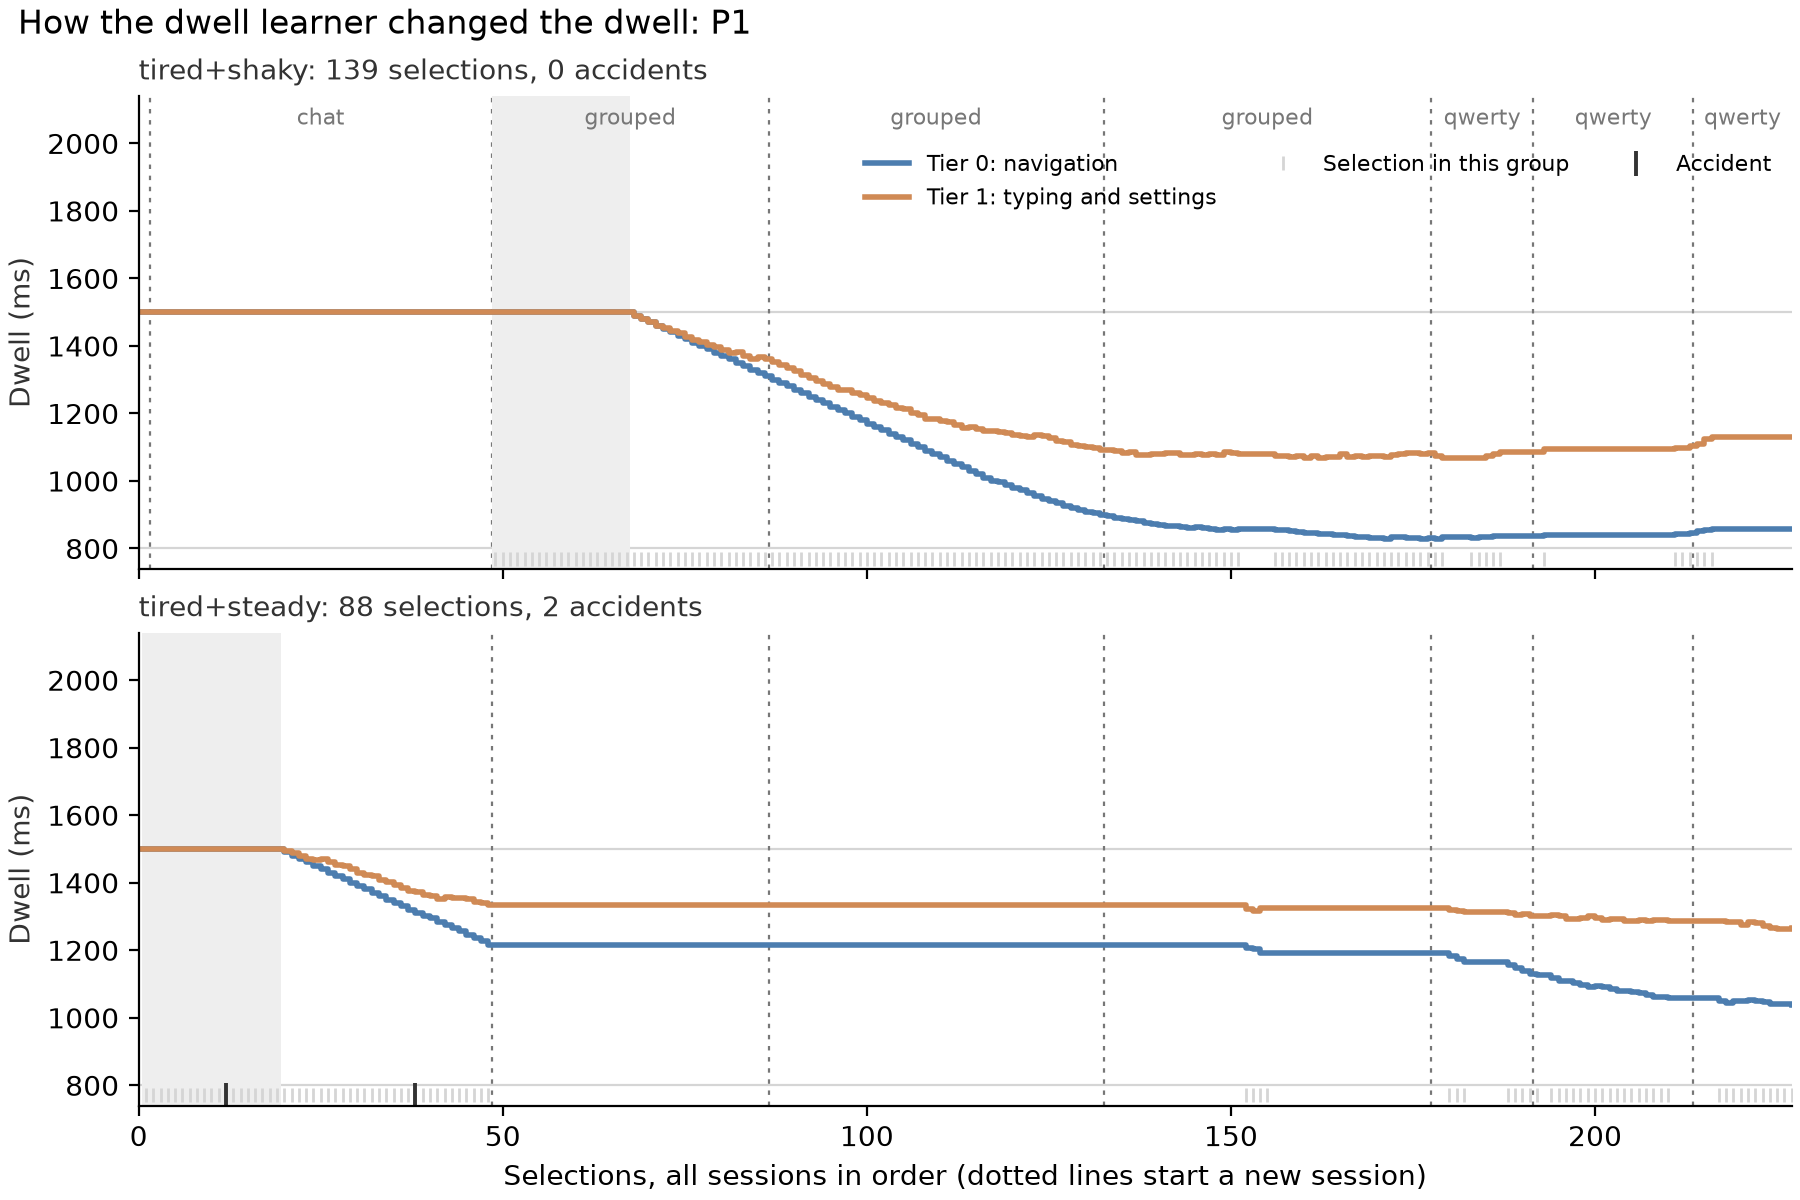
\includegraphics[width=0.85\linewidth]{figures/dwell_p1.png}
  \caption{P1's dwell over all sessions, one panel per context group and one line per tier. The
  shaded area is the warm-up; the first session is the free use session, followed by three
  grouped and three QWERTY typing runs. Marks along the bottom are the group's selections (light)
  and accidents (dark).}
  \Description{Two stacked step plots of dwell time against selection count. In the top panel
  (tired and shaky) both lines stay at 1500 ms until about selection 68, then fall to about
  860 ms for tier 0 and 1130 ms for tier 1. In the bottom panel (tired and steady) the lines fall
  from 1500 ms after selection 20 to about 1216 and 1333 ms, stay flat while the group is not in
  use, and fall further near the end.}
  \label{fig:dwell}
\end{figure}

\begin{table}[t]
  \caption{Typing test, mean of three two minute runs per keyboard. The mean tier 1 dwell in use
  during the runs is shown because the dwell was still learning during this test.}
  \label{tab:typing}
  \small
  \begin{tabular}{llrrrr}
    \toprule
    & Keyboard & WPM & Accuracy & Keystrokes per char. & Mean dwell \\
    \midrule
    \multirow{2}{*}{P1} & Grouped & 2.23 & 100\% & 1.84 & 1261 ms \\
                        & QWERTY  & 1.50 & 91.7\% & 1.06 & 1214 ms \\
    \midrule
    \multirow{2}{*}{P2} & Grouped & 1.60 & 100\% & 1.86 & 1327 ms \\
                        & QWERTY  & 0.57 & 100\% & 1.11 & 1259 ms \\
    \bottomrule
  \end{tabular}
\end{table}

\textbf{Typing.} The grouped keyboard was faster for both participants (Table~\ref{tab:typing}),
by 1.5 times for P1 and 2.8 times for P2, even though it needs almost two selections per letter.
The dwell does not explain this: the mean dwell during the QWERTY runs was slightly shorter than
during the grouped runs. Target size does. On the typing screen a letter group was
316~$\times$~113 px and a QWERTY key 113~$\times$~67 px, while the calibration error was 69 to
80 px, about the height of a QWERTY key. Figure~\ref{fig:heatmap} shows how widely P2's gaze
spread around the targets on the compose screen. Speeds are low in absolute terms, as expected
for first time users with a dwell above one second and no word suggestions.

\begin{figure}[t]
  \centering
  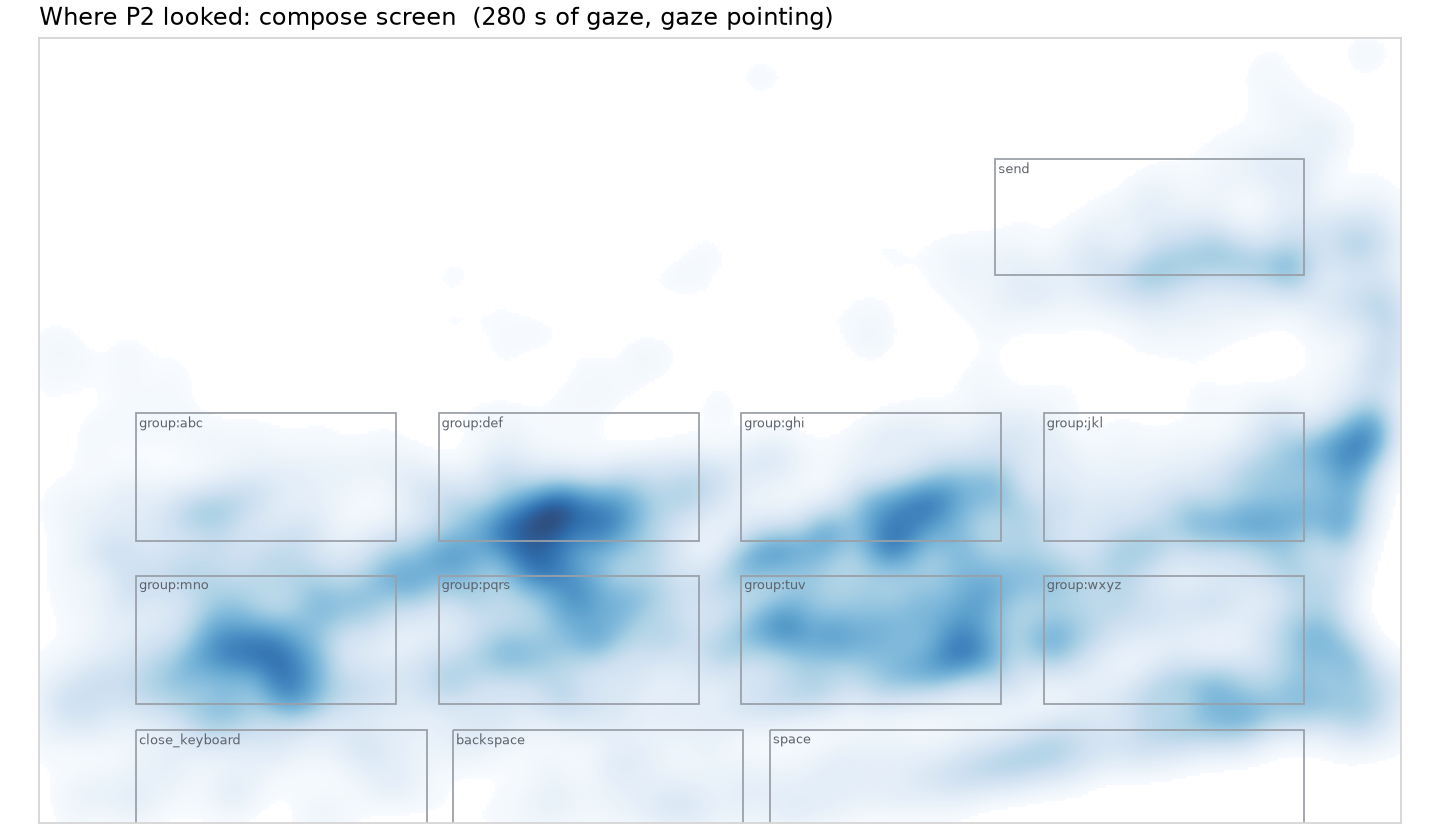
\includegraphics[width=0.75\linewidth]{figures/heatmap_p2_compose.png}
  \caption{Where P2 looked on the compose screen with the grouped keyboard, over the real button
  positions. Gaze spreads well beyond the targets, which favours few, large targets.}
  \Description{A gaze density map over the compose screen. Eight letter group buttons in two rows,
  a Send button at the top right, and Close, Backspace and Space at the bottom. Dense areas sit
  on the def, ghi, mno and tuv groups and spread between and around the buttons.}
  \label{fig:heatmap}
\end{figure}

\section{Discussion and Limitations}

The early data support the design's main bet. Accidents stayed rare and confined to cheap,
undoable actions, while the dwell on those actions came down by about a fifth within one session.
No risky action fired by mistake, and the router began to drop the extra signal on tier 2
for a participant whose confirmations had worked. The typing results suggest that for gaze on a
commodity phone, target size matters more than the number of selections per letter.

These results come from two able-bodied participants with no baseline condition, so they show
that the learners behave as intended, not that adaptation beats a fixed dwell. Three limitations
follow from the data. First, the typing runs were recorded while the dwell was still learning,
and grouped runs always came first; we have since fixed the dwell during the typing test and will
counterbalance the order. Second, our time of day rule treated a session after midnight as
rested; the tired flag should use session length and time awake rather than the clock. Third,
with a 1500 ms start and a 20 selection warm-up, the learner needs about 70 selections to settle,
longer than a short study session.

\textbf{Planned study.} We are extending the study to two more able-bodied participants and one
participant with a motor impairment. Each will use the app twice with gaze pointing, once with
the adaptive learners and once with a fixed baseline (1000 ms dwell, dwell alone on tier 2, the
preferred signal on tier 3), in counterbalanced order, with 5 minutes of practice, the four
tasks, and the System Usability Scale \cite{brooke1996} after each session. We will compare
accidents and give-ups per 100 selections, task times and SUS with paired tests, and report the
participant with a motor impairment as a case study.

\section{Conclusion}

Communic-aid shows that one consumer phone can provide both the pointing and the confirmation
signals for a hands-free messaging interface, and that the interface can learn, from ordinary use
and without asking, how long to wait and which signal to ask for before acting. Treating dwell
and confirmation as two settings of one question, scaled by the cost of an error, gives a simple
way to make gaze interaction both safer and faster for each person.

\bibliographystyle{ACM-Reference-Format}
\bibliography{refs}

\end{document}
